% Created 2020-03-02 Mon 21:13
% Intended LaTeX compiler: pdflatex
\documentclass[table,svgnames,aspectratio=169]{beamer}
\usepackage[utf8]{inputenc}
\usepackage[T1]{fontenc}
\usepackage{graphicx}
\usepackage{grffile}
\usepackage{longtable}
\usepackage{wrapfig}
\usepackage{rotating}
\usepackage[normalem]{ulem}
\usepackage{amsmath}
\usepackage{textcomp}
\usepackage{amssymb}
\usepackage{capt-of}
\usepackage{hyperref}
\usepackage{listings}
% \documentclass[table,aspectratio=169]{beamer}

% This AU beamer theme is based on the beamer theme metropolis
% repo: https://github.com/matze/mtheme
\usetheme{metropolis}

\usepackage[utf8]{inputenc}
\usepackage[absolute,overlay]{textpos}
\usepackage{xspace}
\usepackage{amsmath,amssymb}
\usepackage{graphbox}
\usepackage{epstopdf}
\usepackage{listing}

\usepackage{tikz}
\usepackage{pgfplots}
\pgfplotsset{compat=newest}

\definecolor{AUblue}{rgb}{0.0, 0.37, 0.70} % AU Blue (primary)
\setbeamertemplate{footline}[frame number]      
\setbeamercolor{palette primary}{bg=AUblue,fg=white}

\setbeamertemplate{footline}{%
  \hspace{.5cm}
%  
\includegraphics[align=c, height=.5cm]{graphics/logos/aulogo_uk_var2_blue.eps}
%  \hspace{1cm}
  
\includegraphics[align=c, height=1cm]{graphics/logos/scale_iot.eps}%
  \hspace{1cm}
  
\includegraphics[align=c, height=1cm]{graphics/logos/netx_logo.png}%
  \hfill%
  \usebeamercolor[fg]{page number in head/foot}%
  \usebeamerfont{page number in head/foot}%
  \insertframenumber\,/\,\inserttotalframenumber\kern1em%
}

\setbeamertemplate{frametitle}{\nointerlineskip  
  \begin{beamercolorbox}[wd=\paperwidth,ht=2.75ex,dp=1.375ex]{frametitle}
    \hspace*{2ex}\insertframetitle \hfill  
\includegraphics[align=c, height=.5cm]{graphics/logos/aulogo_uk_var2_white.eps} \hspace*{1ex}%
  \end{beamercolorbox}}      

\setbeamercolor{alerted text}{%
  fg=AUblue,
}
% \input{info}
\usepackage{xcolor}
\lstset{ 
  backgroundcolor=\color{white},   % choose the background color; you must add \usepackage{color} or \usepackage{xcolor}; should come as last argument
  basicstyle=\footnotesize,        % the size of the fonts that are used for the code
  breakatwhitespace=false,         % sets if automatic breaks should only happen at whitespace
  breaklines=true,                 % sets automatic line breaking
  captionpos=b,                    % sets the caption-position to bottom
  commentstyle=\color{mygreen},    % comment style
  deletekeywords={...},            % if you want to delete keywords from the given language
  escapeinside={\%*}{*)},          % if you want to add LaTeX within your code
  extendedchars=true,              % lets you use non-ASCII characters; for 8-bits encodings only, does not work with UTF-8
  firstnumber=1000,                % start line enumeration with line 1000
  frame=single,	                   % adds a frame around the code
  keepspaces=true,                 % keeps spaces in text, useful for keeping indentation of code (possibly needs columns=flexible)
  keywordstyle=\color{blue},       % keyword style
  morekeywords={*,...},            % if you want to add more keywords to the set
  numbers=left,                    % where to put the line-numbers; possible values are (none, left, right)
  numbersep=5pt,                   % how far the line-numbers are from the code
  numberstyle=\tiny\color{mygray}, % the style that is used for the line-numbers
  rulecolor=\color{black},         % if not set, the frame-color may be changed on line-breaks within not-black text (e.g. comments (green here))
  showspaces=false,                % show spaces everywhere adding particular underscores; it overrides 'showstringspaces'
  showstringspaces=false,          % underline spaces within strings only
  showtabs=false,                  % show tabs within strings adding particular underscores
  stepnumber=2,                    % the step between two line-numbers. If it's 1, each line will be numbered
  stringstyle=\color{mymauve},     % string literal style
  tabsize=2,	                   % sets default tabsize to 2 spaces
  title=\lstname                   % show the filename of files included with \lstinputlisting; also try caption instead of title
}
\usetheme{default}
\author{Lars Nielsen}
\date{}
\title{Introduction to Git}
\hypersetup{
 pdfauthor={Lars Nielsen},
 pdftitle={Introduction to Git},
 pdfkeywords={},
 pdfsubject={},
 pdfcreator={Emacs 26.3 (Org mode 9.1.9)}, 
 pdflang={English}}
\begin{document}

{
  \setbeamertemplate{footline}{%
    \hspace{.5cm}
    
\includegraphics[align=c, height=.5cm]{graphics/logos/aulogo_uk_var2_blue.eps}
    \hspace{1cm}
    
\includegraphics[align=c, height=1cm]{graphics/logos/scale_iot.eps}%
    \hspace{1cm}
    
\includegraphics[align=c, height=1cm]{graphics/logos/netx_logo.png}%    
  }
  \begin{frame}[noframenumbering]
    \titlepage
  \end{frame}
}

\begin{frame}[label={sec:org0b52e43}]{Agenda}
TBW
\end{frame}

\begin{frame}[label={sec:org0912c8f}]{Version Control System (VCS)}
\alert{General}

\begin{itemize}
\item Provides a common repository for code
\item A system that lets you keep track of different version of file
\item It allows for traceability
\end{itemize}

\alert{Most} 

\begin{itemize}
\item Enables collaboration
\item Provide merging of files
\end{itemize}

\alert{Some} 

\begin{itemize}
\item Fights collaboration
\item Centralised
\item Distributed
\end{itemize}
\end{frame}

\begin{frame}[label={sec:org723e529}]{VCS - Centralised}
\begin{itemize}
\item There is one repository all works on
\item It is often in a server
\item Some requires file lock and release
\begin{itemize}
\item Some are even worse
\end{itemize}
\end{itemize}
\end{frame}

\begin{frame}[label={sec:org3708ea4}]{VCS - Decentralised}
\begin{itemize}
\item Every computer has a repository
\item \alert{Most} sync to a common base
\end{itemize}
\end{frame}



\begin{frame}[label={sec:orgf084af8}]{Brief History}
\begin{itemize}
\item Released in 2005 (so "young")
\item Create because according to "the git" all other VCS sucked 
\begin{itemize}
\item Especially CVS
\end{itemize}
\item Maintain Juni Hamano
\end{itemize}
\end{frame}

\begin{frame}[label={sec:orgdf5c308}]{Where to get git}
\alert{Linux}

It should be in your package repository (if not switch distro). 


\alert{MacOS}

Should be pre-installed. But is easier to mange with Homebrew 

\alert{Windows} 

It can be downloaded straight from: \url{https://git-scm.com/} 
\end{frame}


\begin{frame}[label={sec:orge7bb416}]{Basic commands}
There are 6 main commands in \emph{git} and it should be the only once you should need in the beginning. 

\begin{itemize}
\item clone
\item add
\item commit
\item push
\item pull
\item status
\end{itemize}
and \emph{checkout}.
\end{frame}

\begin{frame}[fragile,label={sec:org9107b1f}]{Basic Commands - Clone}
 The \emph{clone} command is used for getting a copy of the repository 

\lstset{language=bash,label= ,caption= ,captionpos=b,numbers=none}
\begin{lstlisting}
git clone URI
\end{lstlisting}

\begin{itemize}
\item You get the full version history
\item You get all current branches
\end{itemize}
\end{frame}

\begin{frame}[fragile,label={sec:org747fa41}]{Basic Commands - Add and Commit}
 \lstset{language=bash,label= ,caption= ,captionpos=b,numbers=none}
\begin{lstlisting}
git add [params]
git commit -m "MSG"
\end{lstlisting}

\begin{columns}
\begin{column}[t]{0.5\columnwidth}
\alert{add}
\begin{itemize}
\item adds \texttt{[params]} to a staging area 
\begin{itemize}
\item \texttt{.} \(\rightarrow\) add everything in folder
\item \texttt{*} \(\rightarrow\) add all (just like BASH)
\item \texttt{-u} \(\rightarrow\) add all files all ready tracked
\item \texttt{dir} \(\rightarrow\) add content of the directory dir
\item \texttt{file name} \(\rightarrow\) add a file or files
\end{itemize}
\end{itemize}
\end{column}



\begin{column}[t]{.5\columnwidth}
\alert{commit}
\begin{itemize}
\item Commits a your staging area to the repository history
\item Takes a message 
\begin{itemize}
\item Make it a descriptive message
\end{itemize}
\end{itemize}
\end{column}
\end{columns}
\end{frame}

\begin{frame}[fragile,label={sec:orgadc11c3}]{Basic Commands - Pull and Push}
 \lstset{language=bash,label= ,caption= ,captionpos=b,numbers=none}
\begin{lstlisting}
git pull 
git push 
\end{lstlisting}

\begin{columns}
\begin{column}[t]{0.5\columnwidth}
\alert{pull}
\begin{itemize}
\item Get the history in the base repository
\item Get the branches in the base repository 
\begin{itemize}
\item Depends on the base setup
\end{itemize}
\end{itemize}
\end{column}

\begin{column}[t]{0.5\columnwidth}
\alert{push}
\begin{itemize}
\item Push your changes to the base repo
\item Distribute your changes to others
\end{itemize}
\end{column}
\end{columns}
\end{frame}

\begin{frame}[label={sec:org9336622}]{Basic Commands - Status}
\begin{center}
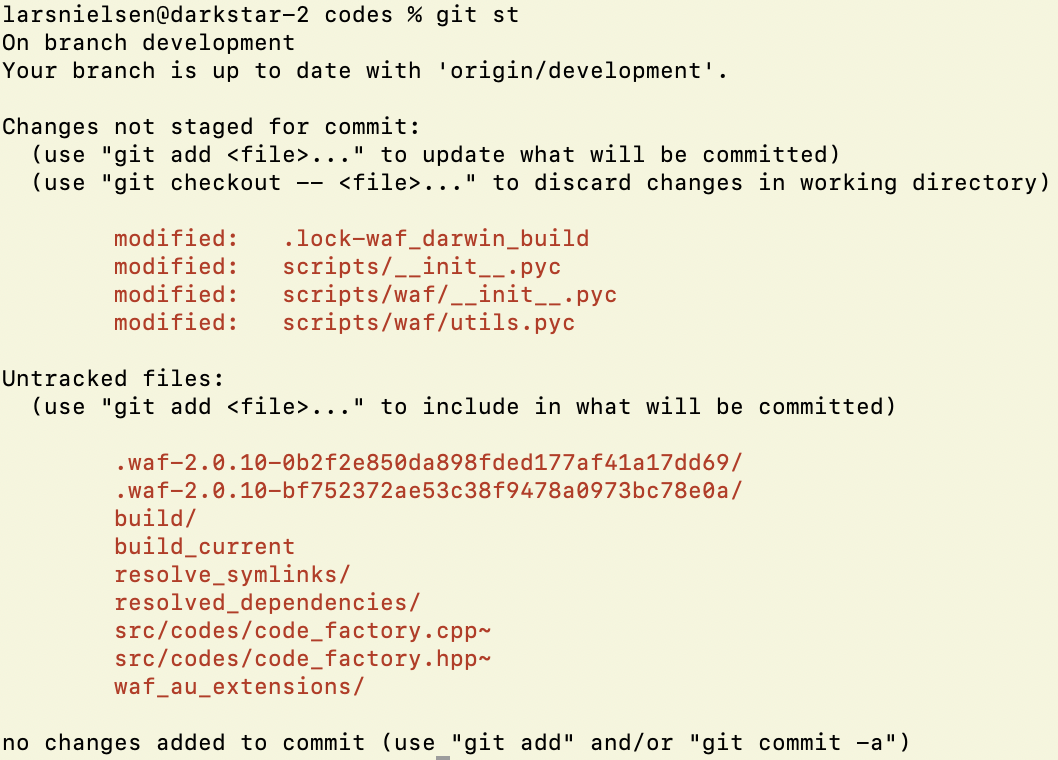
\includegraphics[width=.75\textwidth,height=7cm]{graphics/status.png}
\end{center}
\end{frame}

\begin{frame}[label={sec:orgf19e270}]{Branching}
\begin{columns}
\begin{column}{.5\columnwidth}
\begin{itemize}
\item Separate your work
\item Do not break others code
\item Segment releases
\item All repos are
\item All repos has a master branch
\end{itemize}
\end{column}
\begin{column}{.5\columnwidth}
\begin{center}
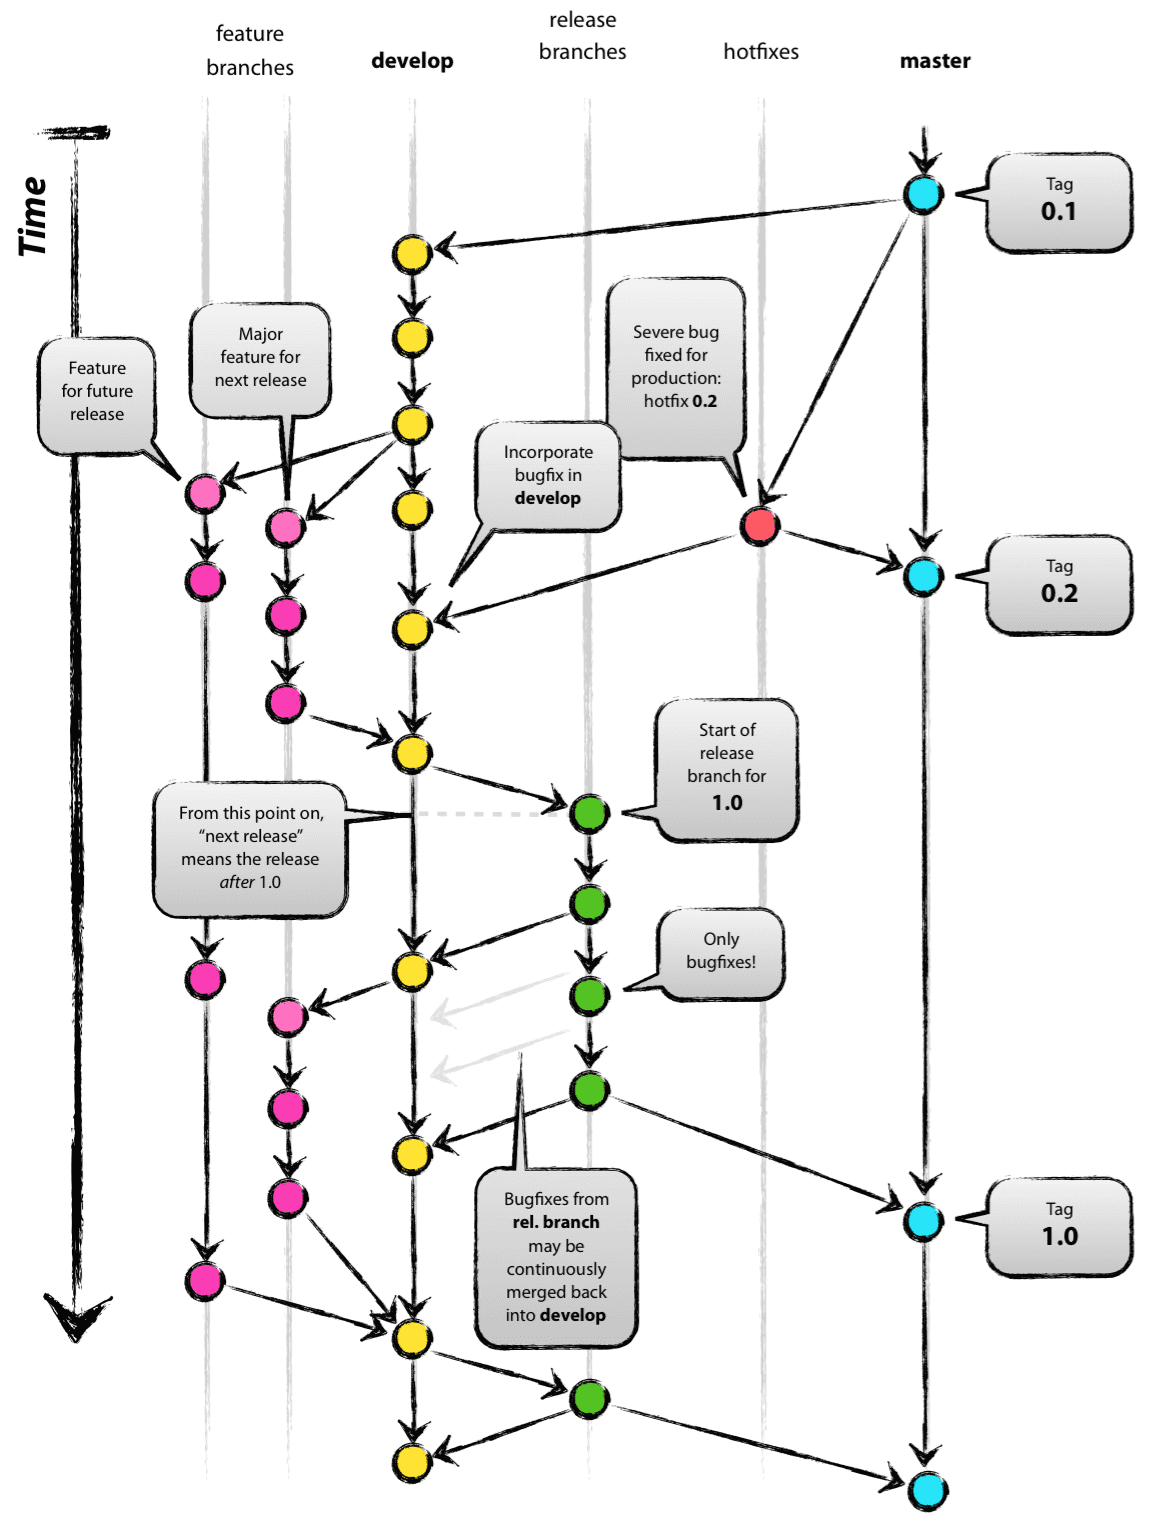
\includegraphics[width=.75\textwidth]{graphics/git-model.png}
\end{center}
\end{column}
\end{columns}
\end{frame}

\begin{frame}[fragile,label={sec:orgb3117a5}]{Working with branches}
 \lstset{language=bash,label= ,caption= ,captionpos=b,numbers=none}
\begin{lstlisting}
git checkout -b NEW_BRANCH_NAME BASE_BRANCH
...
git push -U origin NEW_BRANCH_NAME
\end{lstlisting}

\begin{columns}
\begin{column}{.5\columnwidth}
\begin{center}
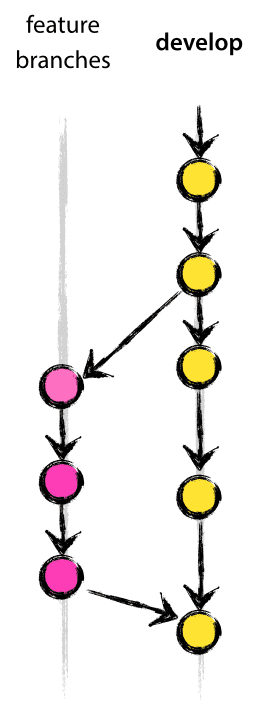
\includegraphics[height=6cm]{graphics/fb2x.png}
\end{center}
\end{column}

\begin{column}{.5\columnwidth}
\begin{itemize}
\item Create a branch
\item work in it, \emph{add}, \emph{commit}, \emph{push}
\item Ensures minimal interference from others
\item Ensures you don't screw up
\end{itemize}
\end{column}
\end{columns}
\end{frame}


\begin{frame}[fragile,label={sec:org487211f}]{Working with branches}
 \lstset{language=bash,label= ,caption= ,captionpos=b,numbers=none}
\begin{lstlisting}
git checkout BASE_BRANCH
git merge NEW_BRANCH_NAME 
git branch -d NEW_BRANCH_NAME 
\end{lstlisting}

\begin{columns}
\begin{column}{.5\columnwidth}
\begin{center}
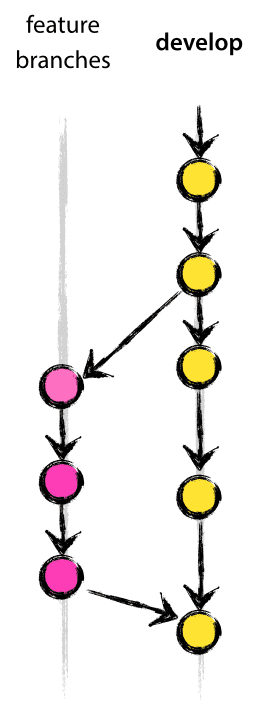
\includegraphics[height=6cm]{graphics/fb2x.png}
\end{center}
\end{column}

\begin{column}{.5\columnwidth}
\begin{itemize}
\item Create a branch
\item work in it, \emph{add}, \emph{commit}, \emph{push}
\item Ensures minimal interference from others
\item Ensures you don't screw up
\end{itemize}
\end{column}
\end{columns}
\end{frame}


\begin{frame}[fragile,label={sec:org8a68cb7}]{Working with branches - the old Switcheroo}
 Some time you may need to switch between branch. 

\lstset{language=bash,label= ,caption= ,captionpos=b,numbers=none}
\begin{lstlisting}
git checkout BRANCH_NAME
\end{lstlisting}
\end{frame}

\begin{frame}[label={sec:org90eca7d}]{Working with branches - Git Flow}
\begin{center}
\href{https://nvie.com/posts/a-successful-git-branching-model/}{https://nvie.com/posts/a-successful-git-branching-model/}
\end{center}
Git flow is a branching model
\end{frame}

\begin{frame}[label={sec:org5af6d69}]{Tagging}
\begin{itemize}
\item Semantic Versioning (not git) \(\rightarrow\) BUT AWESOME
\item It is used for tagging a specific commit
\item Used for traceability
\end{itemize}
\end{frame}

\begin{frame}[label={sec:org3196f61}]{Tagging - Semantic Versioning}
\begin{itemize}
\item A versioning scheme
\item Has three types of release 
\begin{itemize}
\item Major
\item Minor
\item Hotfix
\end{itemize}
\end{itemize}

\begin{center}
\alert{MAJOR.MINOR.HOTFIX}
\end{center}
\end{frame}

\begin{frame}[fragile,label={sec:org9a45915}]{Tagging}
 \begin{itemize}
\item A tag is a "form of a commit"
\item We need to push tags
\end{itemize}

\lstset{language=bash,label= ,caption= ,captionpos=b,numbers=none}
\begin{lstlisting}
git tag -a VERSION -m "MSG"
git push --tag
\end{lstlisting}

\begin{itemize}
\item Easy to depend on externally
\item Easy traceability
\begin{itemize}
\item You can keep a log of your changes
\end{itemize}
\end{itemize}
\end{frame}


\begin{frame}[label={sec:orgf845d22}]{Work flow}
\begin{columns}
\begin{column}{.5\columnwidth}
\begin{itemize}
\item A \emph{master} branch (stable)
\item A \emph{test} branch (stable)
\item A \emph{developer} branch (some what stable)
\item \emph{feature} branches (unstable)
\item \emph{release} branches (stable)
\end{itemize}
\end{column}
\begin{column}{.5\columnwidth}
\begin{center}
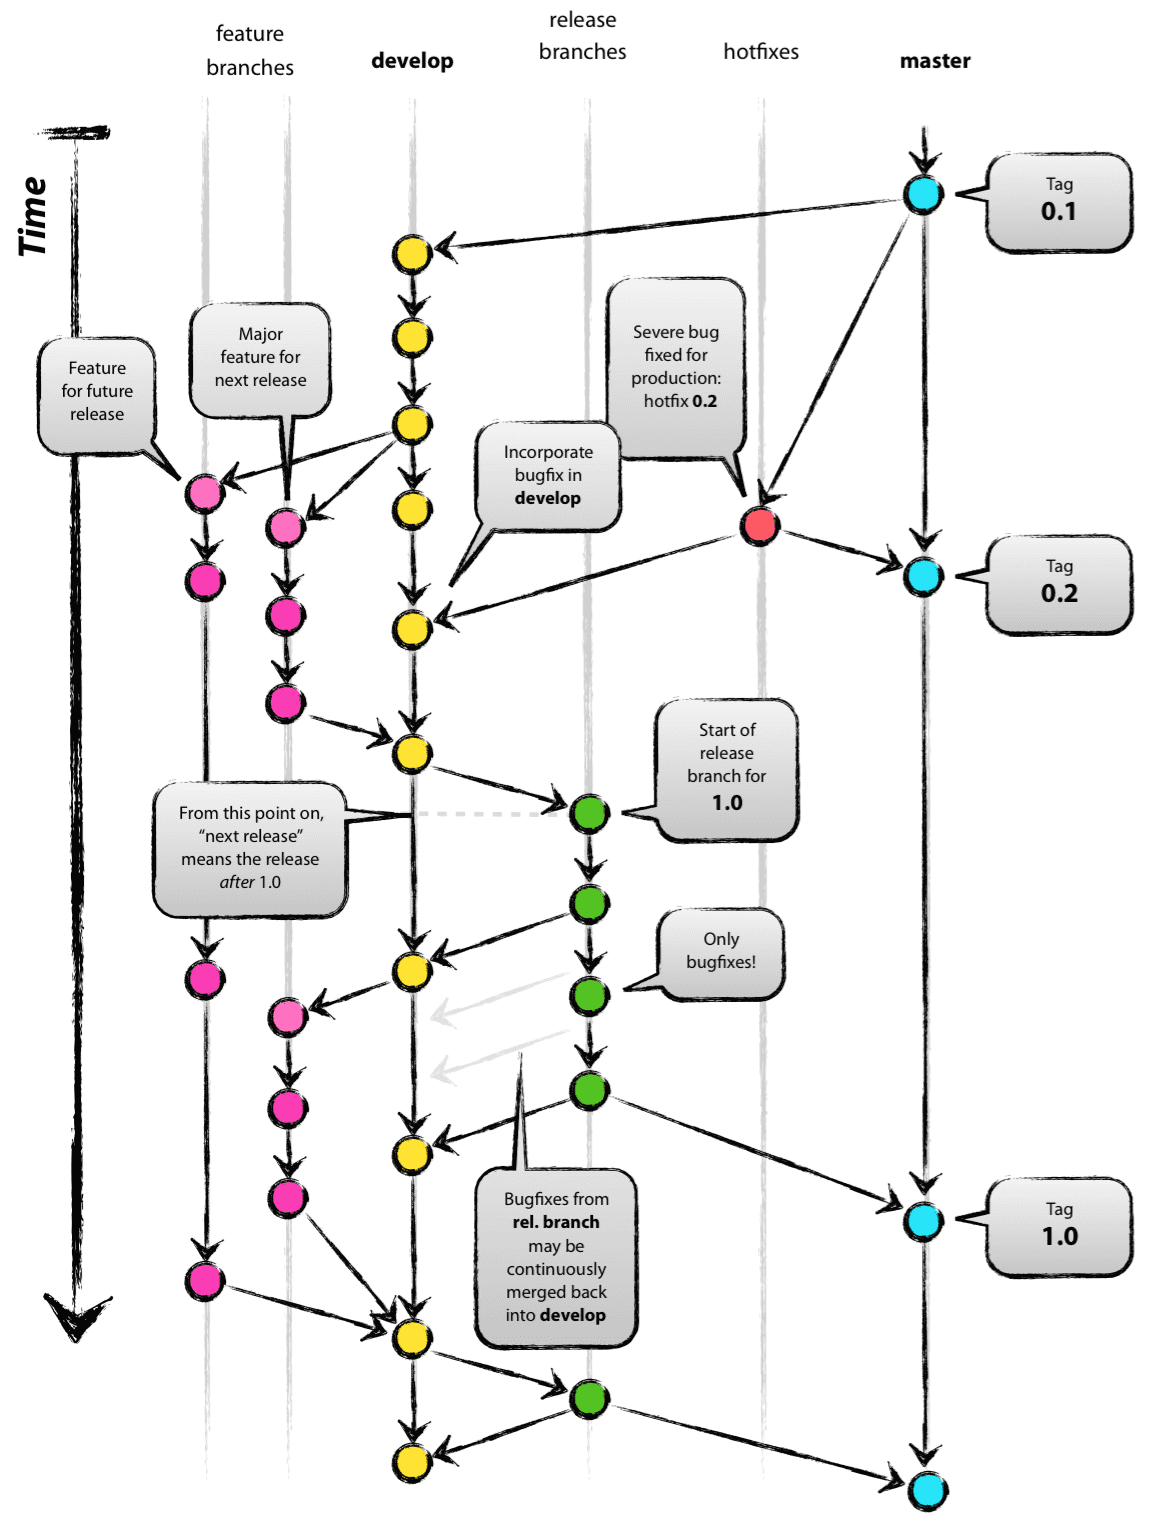
\includegraphics[width=.75\textwidth]{graphics/git-model.png}
\end{center}
\end{column}
\end{columns}
\end{frame}


\begin{frame}[label={sec:org0abef3e}]{Pull Request}
\begin{itemize}
\item A way to
\begin{itemize}
\item Comment on merges
\item Reject a merge
\item Do code review
\end{itemize}
\item Has different names
\begin{itemize}
\item Pull Request
\item Merge request
\item Review request
\end{itemize}
\end{itemize}
\end{frame}

\begin{frame}[label={sec:orgcca262e}]{Hooks}
\begin{columns}
\begin{column}{.5\columnwidth}
\begin{itemize}
\item Magic little "programs"
\item Fine grained control
\item Can be annoying
\item Placed in .git/hooks
\end{itemize}
\end{column}

\begin{column}{.5\columnwidth}
\begin{center}

\includegraphics[width=.5\textwidth]{graphics/hook.jpg}
\end{center}
\end{column}
\end{columns}
\end{frame}


\begin{frame}[fragile,label={sec:org07c060e}]{Hooks}
 \begin{columns}
\begin{column}{.4\columnwidth}
\begin{itemize}
\item "Altering" commands
\item You can change before and after
\item Can be any scripting language you have an execution ENV for
\end{itemize}
\end{column}

\begin{column}{.6\columnwidth}
\lstset{language=bash,label= ,caption= ,captionpos=b,numbers=none}
\begin{lstlisting}
   if [ "$allownonascii" != "true" ] &&
   test $(git diff --cached --name-only --diff-filter=A -z $against |
   LC_ALL=C tr -d '[ -~]\0' | wc -c) != 0
then
        cat <<\EOF
Error: ERROR MSG
EOF
        exit 1
fi


\end{lstlisting}
\end{column}
\end{columns}
\end{frame}

\begin{frame}[label={sec:orgd05de07}]{Hooks - Types}
\begin{itemize}
\item Server Side
\begin{itemize}
\item pre-receive 
\begin{itemize}
\item linting
\item user verification
\end{itemize}
\end{itemize}
\item Client Side 
\begin{itemize}
\item pre-commit
\begin{itemize}
\item linting
\end{itemize}
\end{itemize}
\end{itemize}

\url{https://git-scm.com/book/en/v2/Customizing-Git-Git-Hooks}
\end{frame}

\begin{frame}[fragile,label={sec:orgdb0b6ba}]{.gitingore}
 \begin{columns}
\begin{column}{.5\columnwidth}
\lstset{language=bash,label= ,caption= ,captionpos=b,numbers=none}
\begin{lstlisting}
filename.extension 
foldername/
entry*.extension
entry~
\end{lstlisting}
\end{column}


\begin{column}{.5\columnwidth}
\begin{itemize}
\item Makes files ignored when added
\item can be added with \emph{-f}
\item used for keeping the repo clean
\item used for making the repo "safe"
\end{itemize}
\end{column}
\end{columns}
\end{frame}

\begin{frame}[fragile,label={sec:orgb023bb9}]{Git Config}
 \begin{columns}
\begin{column}{.5\columnwidth}
\begin{itemize}
\item File called \emph{.gitconfig}
\begin{itemize}
\item On macOS, BSD, and Linux in user root
\end{itemize}
\item Allows: 
\begin{itemize}
\item configuring name and email
\item setting editor
\item aliasing
\item setting push and pull style
\item and more
\end{itemize}
\end{itemize}
\end{column}
\begin{column}{.5\columnwidth}
\lstset{language=bash,label= ,caption= ,captionpos=b,numbers=none}
\begin{lstlisting}
[push]
        default = simple
[user]
        name = Lars Nielsen
        email = lnc13.lars@gmail.com
[alias]
        ...
        st = status
        ps = push
        pl = pull
        cb = checkout -b
        psu = push -u origin
        ... 
[core]
        editor = emacs

\end{lstlisting}
\end{column}
\end{columns}
\end{frame}
\begin{frame}[fragile,label={sec:org30fd9bd}]{Tools - Git Interactive}
 \lstset{language=bash,label= ,caption= ,captionpos=b,numbers=none}
\begin{lstlisting}
git commit --interactive
\end{lstlisting}

\begin{center}
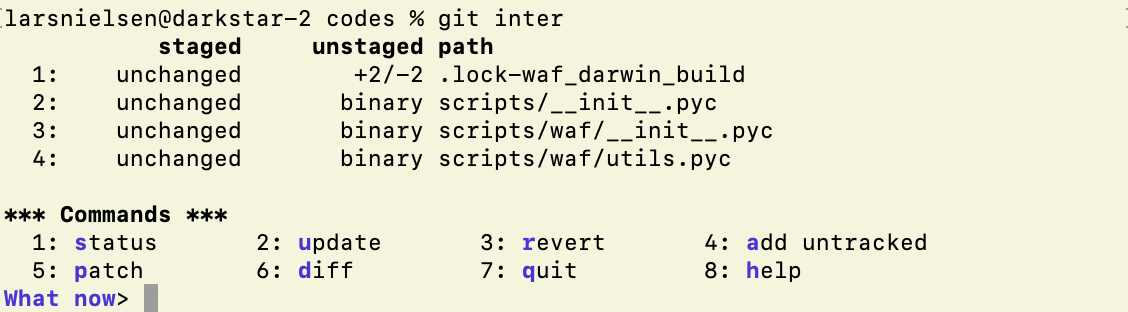
\includegraphics[width=\textwidth]{graphics/interactive.png}
\end{center}
\end{frame}

\begin{frame}[label={sec:orgfcaecc0}]{Tools - Online Repositories}
\begin{columns}
\begin{column}{.33\columnwidth}
\begin{center}

\includegraphics[width=.9\linewidth]{graphics/github.png}
\end{center}
\begin{center}
www.github.com
\end{center}
\end{column}
\begin{column}{.33\columnwidth}
\begin{center}

\includegraphics[width=.9\linewidth]{graphics/bitbucket.jpg}
\end{center}
\begin{center}
www.bitbucket.com
\end{center}
\end{column}

\begin{column}{.33\columnwidth}
\begin{center}

\includegraphics[width=.9\linewidth]{graphics/gitlab.png}
\end{center}
\begin{center}
www.gitlab.com
\end{center}
\end{column}
\end{columns}
\end{frame}


\begin{frame}[label={sec:org6acf1e8}]{Tools - GUI / Mistakes}
\begin{center}
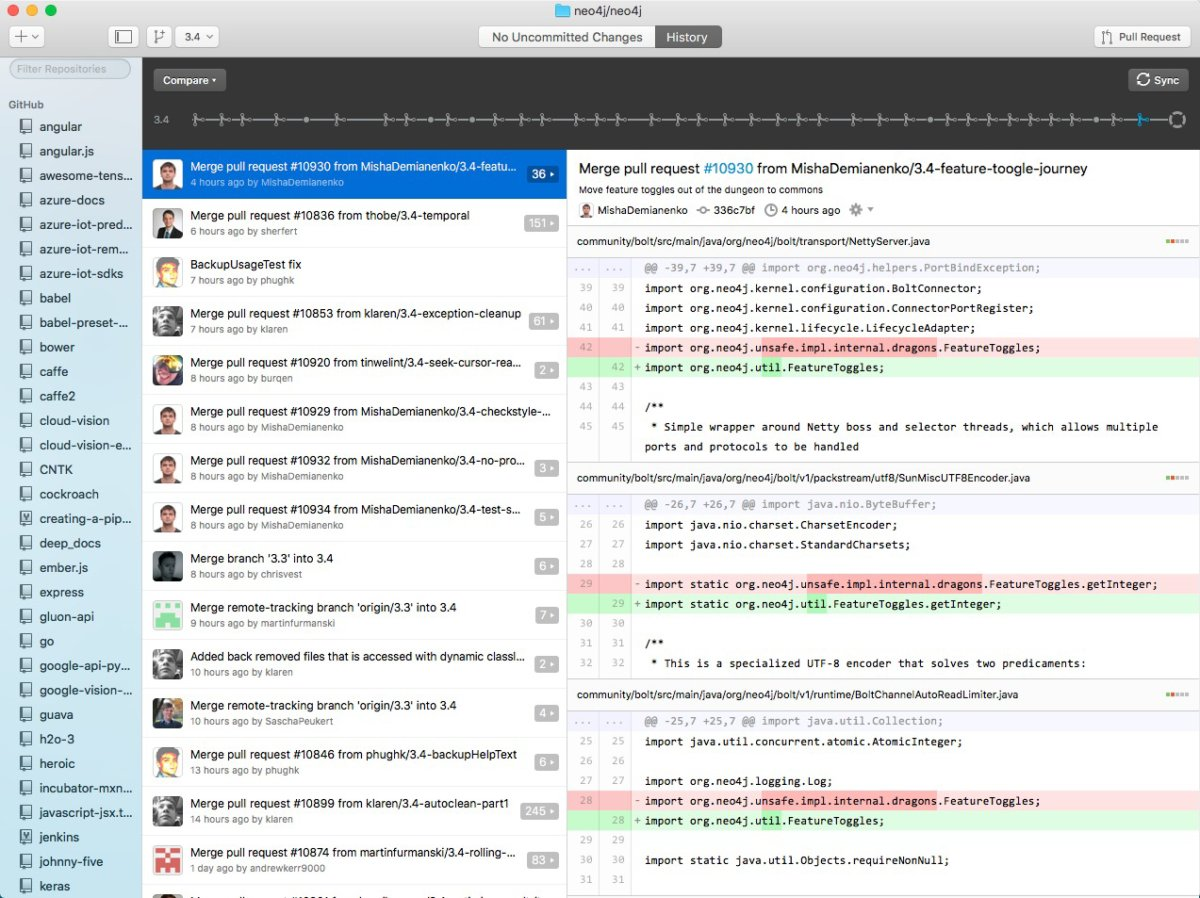
\includegraphics[width=.5\textwidth]{graphics/github_desktop.jpg}
\end{center}

\begin{center}
\url{https://desktop.github.com/}
\end{center}
\end{frame}

\begin{frame}[label={sec:org8146568}]{Tools - Magit}
\begin{columns}
\begin{column}{.5\columnwidth}
\begin{center}

\includegraphics[width=.9\linewidth]{graphics/magit.png}
\end{center}
\end{column}

\begin{column}{.5\columnwidth}
\begin{itemize}
\item Magit
\item Emacs
\item Marius Vollmer, Jonas Bernoulli, etc.
\end{itemize}

\begin{center}
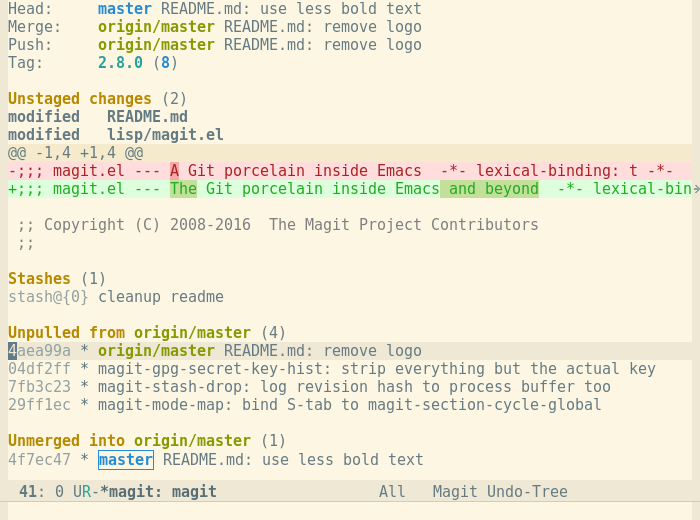
\includegraphics[width=.9\linewidth]{graphics/magit_status.png}
\end{center}
\end{column}
\end{columns}
\end{frame}

\begin{frame}[label={sec:orgc17609f}]{References - Pro Git}
\begin{columns}
\begin{column}{.5\columnwidth}
\begin{center}

\includegraphics[width=.75\textwidth]{graphics/progit2.png}
\end{center}
\end{column}

\begin{column}{.5\columnwidth}
Pro Git

Scott Chacon and Ben Straub 

Free: \url{https://git-scm.com/book/en/v2}

Physical by Apress
\end{column}
\end{columns}
\end{frame}


\begin{frame}[label={sec:orgf4fc788}]{References - Git Pocket Guide}
\begin{columns}
\begin{column}{.5\columnwidth}
Git Pocket Guide

Richard E. Silverman 

O'REILLY 
\end{column}

\begin{column}{.5\columnwidth}
\begin{center}

\includegraphics[height=6cm]{graphics/pocket.jpg}
\end{center}
\end{column}
\end{columns}
\end{frame}
\end{document}